\section{Benutzungsoberfläche}


\subsection{Sartfenster}

\begin{figure}[htbp] 
  \centering
     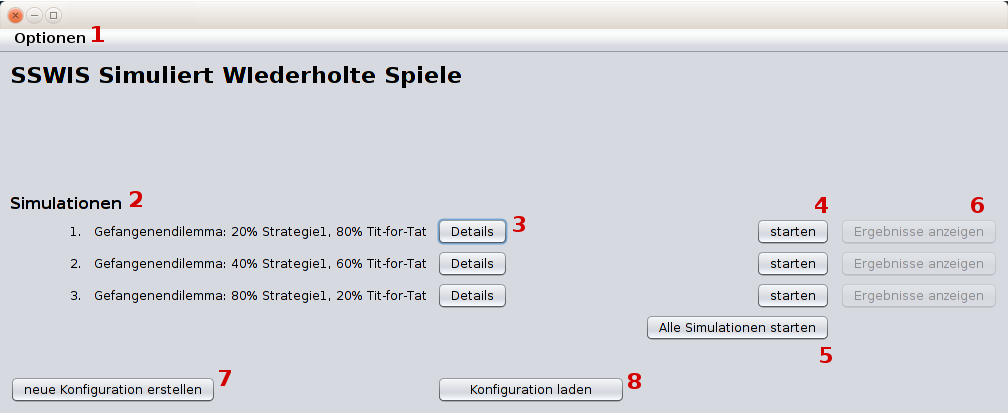
\includegraphics[width=1.2\textwidth]{GUI_Entwurf/StartfensterBeispiel.png}
  \caption{Entwurf}
  \label{fig:Bild1}
\end{figure}

\begin{description}


\item[1. Optionen] Menü enthält Zwei Untermenüs, Ergebnisse und Konfigurationen über die gespeicherte Ergebnisse und Startkonfigurationen angezeigt werden können

\item[2. Simulationen] Liste der geladenen Simulationen. Die wichtigsten Startkonfigurationen wie das Stufenspiel und die gewählten Strategien werden angezeigt.

\item[3. Details] Über diesen Knopf kann in einem Pop-Up-Fenster alle Parameter der Startkonfiguration eingesehen werden.

\item[4. starten] Die jeweilige Simulation kann über diesen Knopf ausgeführt werden. Wird die Simulation bereits ausgeführt oder ist sie in der Warteschlange, so ist der Knopf deaktiviert.

\item[5. Alle Simulationen starten] Durch diesen Knopf werden alle Simulationen, die nicht gerade ausgeführt oder bereits in der Warteschlange sind, nach einander ausgeführt. 

\item[6. Ergebnisse anzeigen] Bei Betätigung werden die Ergebnisse der jeweiligen Simulation der letzen Ausführung angezeigt. Wurde die Simulation noch nicht ausgeführt, ist der Knopf deaktiviert.

\item[7. neue Konfiguration erstellen] Führt zum Assistenten, um alle Parameter für eine neue Startkonfiguration zu bestimmen.

\item[8. Konfiguration laden] Öffnet ein Dialogfenster, in dem man eine zuvor gespeicherte Konfiguration auswählen kann.

\end{description}


\subsection{Konfigurationen erstellen}

\begin{figure}[htbp] 
  \centering
     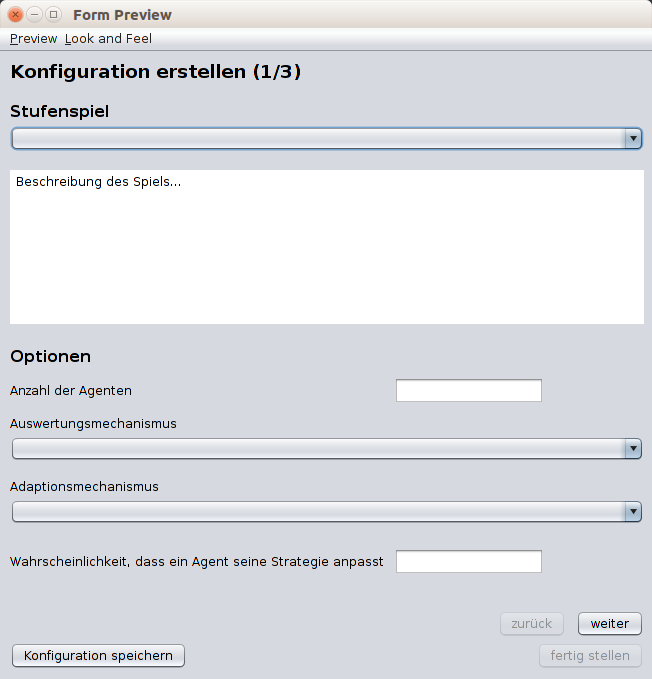
\includegraphics[width=1.0\textwidth]{GUI_Entwurf/WizardFenster1.png}
  \caption{Entwurf}
  \label{fig:Bild1}
\end{figure}

\begin{description}

\item[1. Stufenspiel] Es kann ein Stufenspiel gewählt werden

\item[2. Beschreibung des Spiels] Wenn ein Stufenspiel gewählt ist, steht hier eine kurze Beschreibung unteranderem mit den unterschiedlichen Auszahlungen

\item[3. Anzahl der Agenten] Es werden nur gerade Zahlen akzeptiert

\item[4. Auswertungsmechanismus] Es kann zwischen den Auswertungsmechanismen gewählt werden.

\item[5. Adaptionsmechanismus] Es kann zwischen den Adaptionsmechanismen gewählt werden.

\item[6. Wahrscheinlichkeit] Hier kann eine Wahrscheinlichkeit größer als null und kleiner gleich 100 in Prozent angegeben werden, dass Agenten nach einem Zyklus ihre Startegie gegebenen falls anpassen.

\item[7. Konfiguration speichern] Es öffnet sich ein Dialogfenster, um einen Namen für die erstellt Konfiguration zu bestimmen.

\item[8. zurück] Ist auf dieser Seite deaktiviert.

\item[9. weiter] Führt zur nächsten Seite, wenn alle Parameter korrekt eingegeben wurden. Bei falschen oder fehlenden Eingaben gibt es eine Fehlermeldung.

\item[10. fertig stellen] Ist aktiviert wenn alle nötigen Eingaben auf dieser und den anderen zwei Seiten getätigt wurden. Wenn alle Eingaben korrekt sind, wird das Fenster geschlossen und die Simulationen werden auf die Startseite geladen. Bei falschen oder fehlenden Eingaben gibt es eine Fehlermeldung.

\end{description}

\begin{figure}[htbp] 
  \centering
     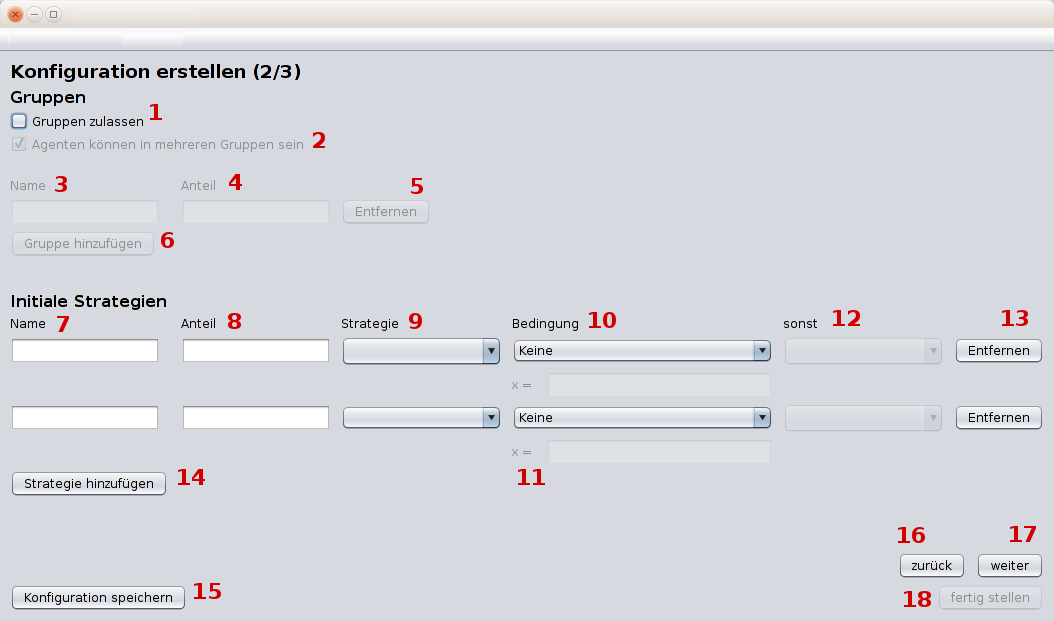
\includegraphics[width=1.2\textwidth]{GUI_Entwurf/WizardFenster2.png}
  \caption{Entwurf}
  \label{fig:Bild1}
\end{figure}

\begin{description}

\item[1. Gruppen zulassen] Aktiviert die Felder 2 bis 6 und aktiviert Bedingung die sich auf Gruppen beziehen.

\item[2. Agenten können in mehreren Gruppen sein] Lässt Überlappungen von Gruppen zu.

\item[3. Name] Name der Gruppe.

\item[4. Anteil] Anteil der Agenten in dieser Gruppe zu Beginn des Spiels in Prozent. Es werden Eingaben größer als null und kleiner gleich 100 akzeptiert.

\item[5. Entfernen] Es kann zwischen den Adaptionsmechanismen gewählt werden.

\item[6. Gruppe hinzufügen] Hier kann eine Wahrscheinlichkeit größer als null und kleiner gleich 100 in Prozent angegeben werden, dass Agenten nach einem Zyklus ihre Startegie gegebenen falls anpassen.

\item[7. Name] Es kann ein Stufenspiel gewählt werden

\item[8. Anteil] Wenn ein Stufenspiel gewählt ist, steht hier eine kurze Beschreibung unteranderem mit den unterschiedlichen Auszahlungen

\item[9. Strategie] Es werden nur gerade Zahlen akzeptiert

\item[10. Bedingung] Es kann zwischen den Auswertungsmechanismen gewählt werden.

\item[11. x] Es kann zwischen den Adaptionsmechanismen gewählt werden.

\item[12. sonst] Hier kann eine Wahrscheinlichkeit größer als null und kleiner gliech 100 in Prozent angegeben werden, dass Agenten nach einem Zyklus ihre Startegie gegebenen falls anpassen.

\item[13. entfernen] Es kann ein Stufenspiel gewählt werden

\item[14. Strategie hinzufügen] Fügt eine neue Zeile an, mit den Feldern 7 bis 13.

\item[15. Konfiguration speichern] Es öffnet sich ein Dialogfenster, um einen Namen für die erstellt Konfiguration zu bestimmen.

\item[16. zurück] Führt zu der ersten Seite.

\item[17. weiter] Führt zur nächsten Seite, wenn alle Parameter korrekt eingegeben wurden. Bei falschen oder fehlenden Eingaben gibt es eine Fehlermeldung.

\item[18. fertig stellen] Ist aktiviert wenn alle nötigen Eingaben auf dieser und den anderen zwei Seiten getätigt wurden. Wenn alle Eingaben korrekt sind, wird das Fenster geschlossen und die Simulationen werden auf die Startseite geladen. Bei falschen oder fehlenden Eingaben gibt es eine Fehlermeldung.

\end{description}

\begin{figure}[htbp] 
  \centering
     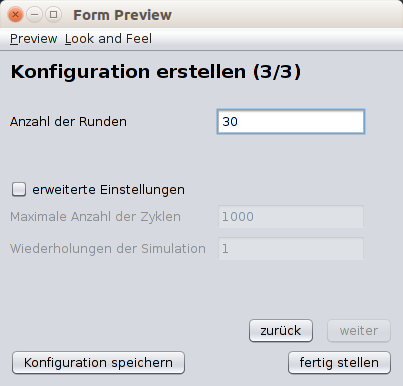
\includegraphics[width=0.7\textwidth]{GUI_Entwurf/WizardFenster3.png}
  \caption{Entwurf}
  \label{fig:Bild1}
\end{figure}


\subsection{Konfigurationen speichern und laden}

\begin{figure}[htbp] 
  \centering
     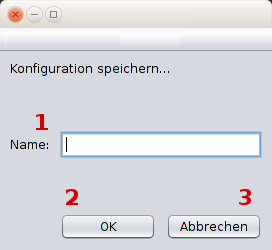
\includegraphics[width=0.5\textwidth]{GUI_Entwurf/KonfigSpeichern.png}
  \caption{Entwurf}
  \label{fig:Bild1}
\end{figure}

\begin{figure}[htbp] 
  \centering
     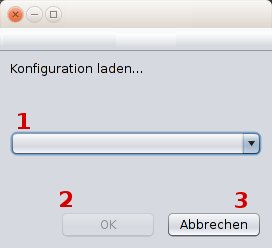
\includegraphics[width=0.5\textwidth]{GUI_Entwurf/KonfigLaden.png}
  \caption{Entwurf}
  \label{fig:Bild1}
\end{figure}



\subsection{Ergebnisse anzeigen}

\begin{figure}[htbp] 
  \centering
     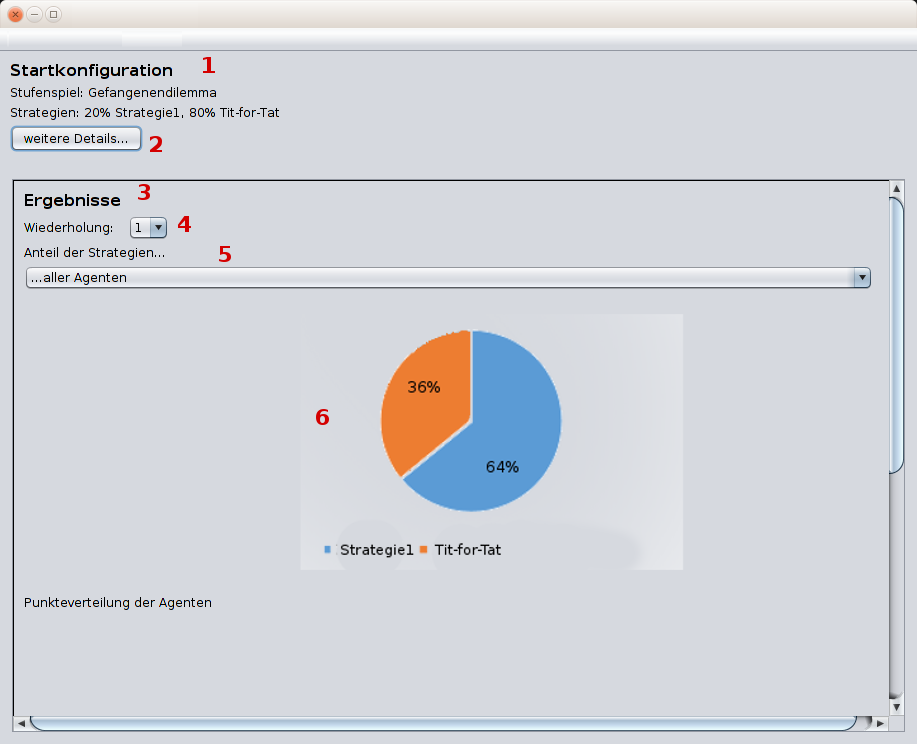
\includegraphics[width=1.2\textwidth]{GUI_Entwurf/Ergebnisfenster1.png}
  \caption{Entwurf}
  \label{fig:Bild1}
\end{figure}


\begin{figure}[htbp] 
  \centering
     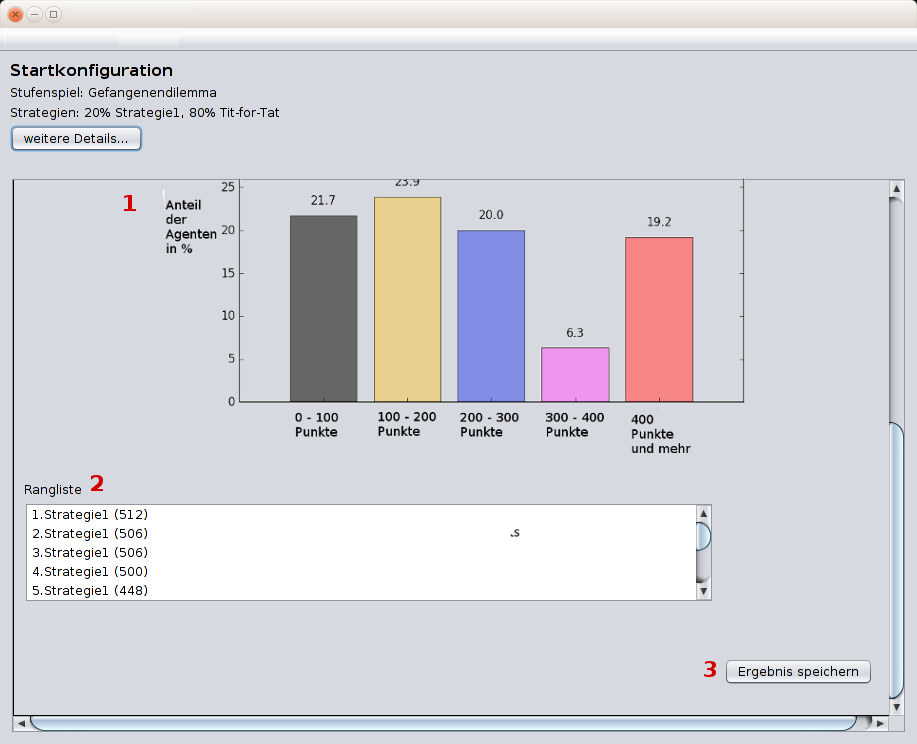
\includegraphics[width=1.2\textwidth]{GUI_Entwurf/Ergebnisfenster2.png}
  \caption{Entwurf}
  \label{fig:Bild1}
\end{figure}

